\documentclass[11pt]{article}

\author{Math 123}
\date{Due March 16, 2023 by midnight} 
\title{Homework 7}

\usepackage{graphicx,xypic}
\usepackage{amsthm}
\usepackage{amsmath,amssymb}
\usepackage{amsfonts}
\usepackage{xcolor}
\usepackage[margin=1in]{geometry}
\usepackage[shortlabels]{enumitem}
\newtheorem{problem}{Problem}
\renewcommand*{\proofname}{{\color{blue}Solution}}


\usepackage{fancyhdr}
\pagestyle{fancy}
\rhead{Math 123, Homework 7}

\setlength{\parindent}{0pt}
\setlength{\parskip}{1.25ex}

% tikz
\usepackage{tikz}
\usetikzlibrary{intersections, angles, quotes, positioning}
\usetikzlibrary{arrows.meta}
\usepackage{pgfplots}
\pgfplotsset{compat=1.13}


\tikzset{
	force/.style={thick, {Circle[length=2pt]}-stealth, shorten <=-1pt}
}

% quiver style
\usepackage{tikz-cd}
% `calc` is necessary to draw curved arrows.
\usetikzlibrary{calc}
% `pathmorphing` is necessary to draw squiggly arrows.
\usetikzlibrary{decorations.pathmorphing}

% A TikZ style for curved arrows of a fixed height, due to AndréC.
\tikzset{curve/.style={settings={#1},to path={(\tikztostart)
					.. controls ($(\tikztostart)!\pv{pos}!(\tikztotarget)!\pv{height}!270:(\tikztotarget)$)
					and ($(\tikztostart)!1-\pv{pos}!(\tikztotarget)!\pv{height}!270:(\tikztotarget)$)
					.. (\tikztotarget)\tikztonodes}},
	settings/.code={\tikzset{quiver/.cd,#1}
			\def\pv##1{\pgfkeysvalueof{/tikz/quiver/##1}}},
	quiver/.cd,pos/.initial=0.35,height/.initial=0}

% TikZ arrowhead/tail styles.
\tikzset{tail reversed/.code={\pgfsetarrowsstart{tikzcd to}}}
\tikzset{2tail/.code={\pgfsetarrowsstart{Implies[reversed]}}}
\tikzset{2tail reversed/.code={\pgfsetarrowsstart{Implies}}}
% TikZ arrow styles.
\tikzset{no body/.style={/tikz/dash pattern=on 0 off 1mm}}

\begin{document}

\maketitle

% You are required to put your name here:
{\bf\Large Name: George Chemmala} 


\vspace{.3in}
Topics covered: Graph coloring, chromatic polynomial, Turan graphs

Instructions: 
\begin{itemize}
\item This assignment must be submitted on Gradescope by the due date. 
\item If you collaborate with other students (which is encouraged!), please mention this somewhere on the assignment. 
\item If you are stuck, please ask for help (from me, a TA, a classmate). Use Campuswire!  
\item You may freely use any fact proved in class. In general, you should provide proof for facts used that were not proved in class. 
\item Please restrict your solution to each problem to a single page. Usually solutions can be even shorter than that. If your solution is very long, you should think more about how to express it concisely.
\end{itemize}


\pagebreak 


\begin{problem}
Give an example or explain why no example exists: A graph $G$ that is neither complete nor an odd cycle, but for which the greedy coloring uses $\Delta(G)+1$ colors. 
\end{problem}

\begin{proof}

\end{proof}

\pagebreak

\begin{problem}
Give a very short proof that the following two graphs have the same chromatic number.\footnote{Note: solutions that construct optimal colorings of these graphs will not receive credit.}
\begin{center}
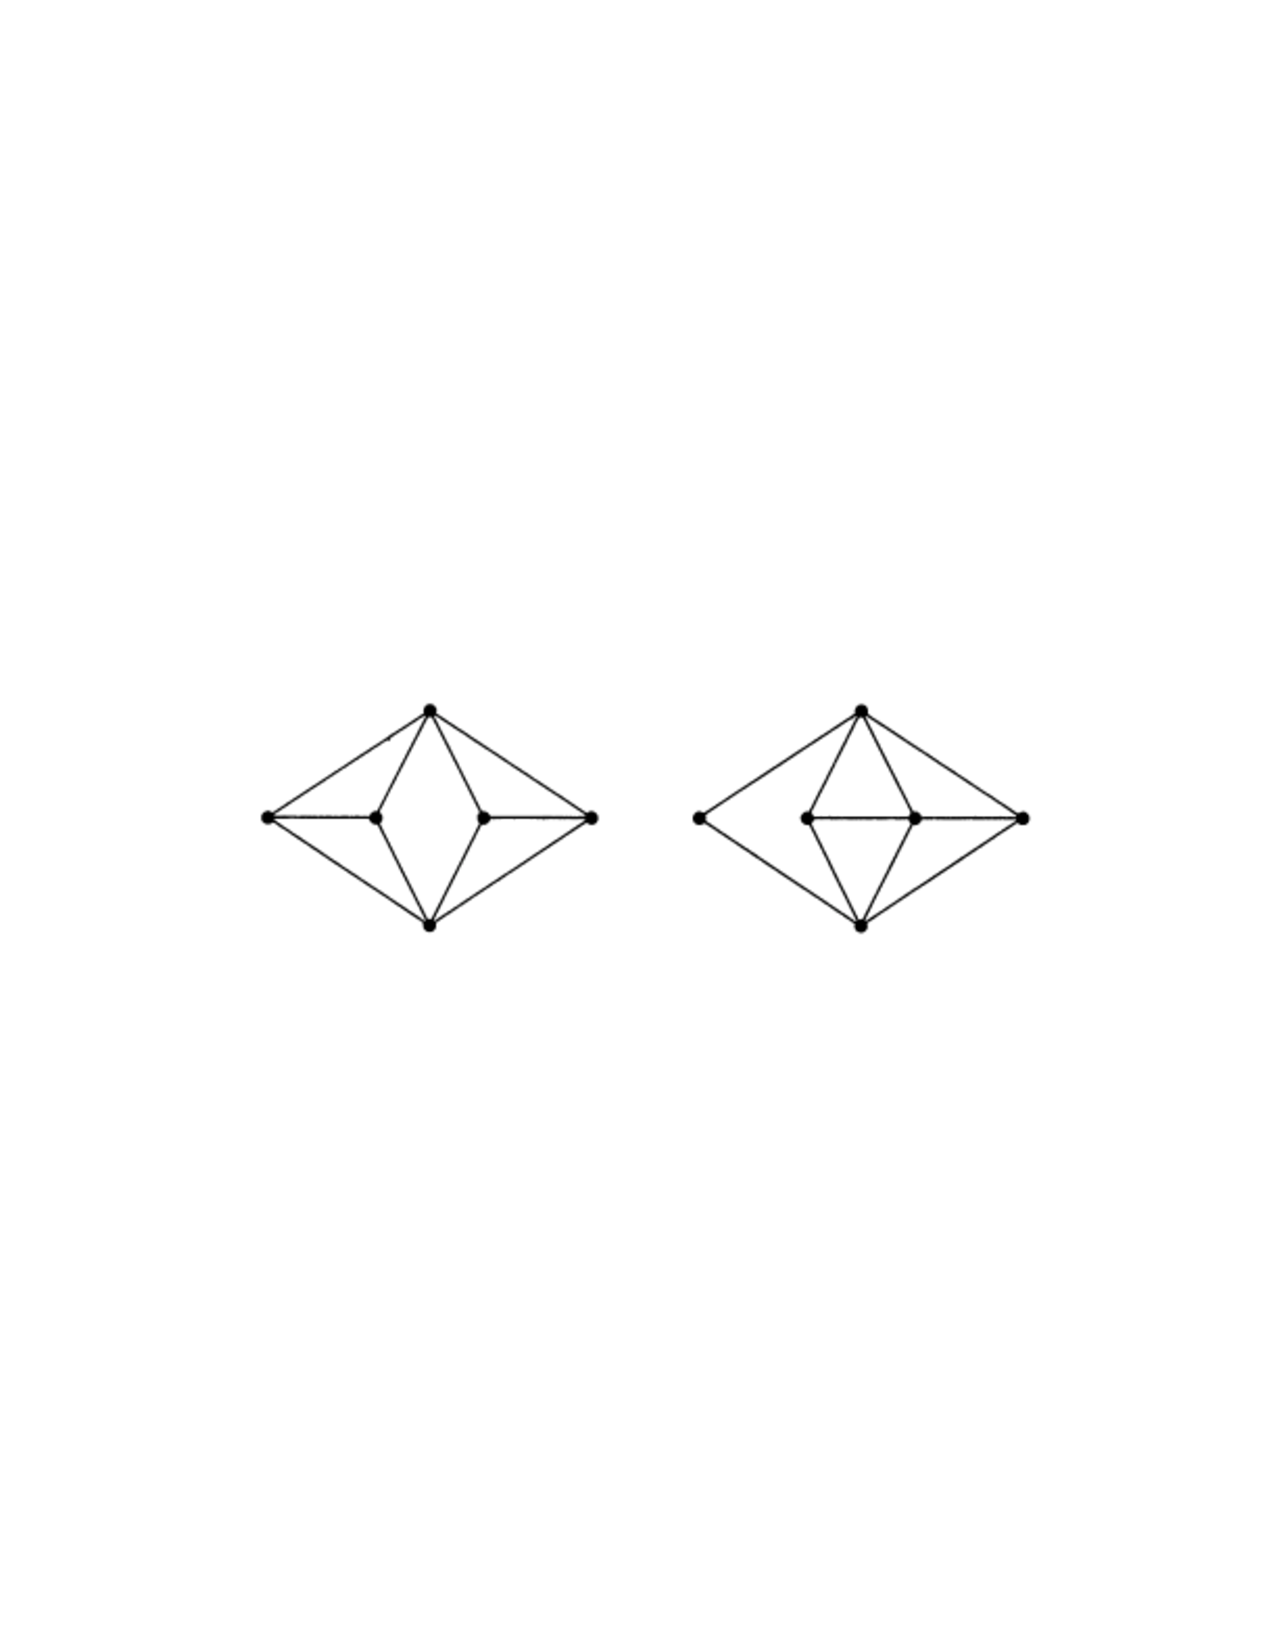
\includegraphics[scale=.5]{hw7-graph.pdf}
\end{center}
\end{problem}

\begin{proof}

\end{proof}

\pagebreak


\begin{problem}
Let $G=M_{n_1,\ldots,n_k}$ be a complete $k$-partite graph with $n=n_1+\cdots+n_r$ vertices. Show that if $n_i-n_j\ge2$ for some $i,j$, then there exists a $k$-partite graph with $n$ vertices and more edges than $G$. 
\end{problem}

\begin{proof}

\end{proof}


\pagebreak


\begin{problem}
Given a set of lines in the plane with no three meeting at a point, form a graph $G$ whose vertices are the intersections of the lines, with two vertices adjacent if they appear consecutively on one of the lines. Prove that $\chi(G)\le3$. 
\footnote{Suggestion: start by looking at some explicit examples.} \footnote{Hint: use a greedy coloring with an appropriate vertex ordering.} 
\end{problem}

\begin{proof}

\end{proof}


\pagebreak



\begin{problem}
Let $G$ be a graph with chromatic number $k$. Show that for every $k$-coloring of $G$ and for each color $i$, there is a vertex of color $i$ that is adjacent to vertices of the other $k-1$ colors. \footnote{Hint: think back to the proof that a graph with chromatic number $k$ has at least ${k\choose 2}$ edges.}
\end{problem}

\begin{proof}

\end{proof}

\pagebreak

\begin{problem}
Prove that $\chi(G)=\omega(G)$ when the complement $\bar G$ is bipartite. \footnote{Here $\omega(G)$ is the clique number: the largest $m$ so that $G$ contains $K_m$.} \footnote{Hint: look to apply K\"onig's theorem. (!)}
\footnote{This is a pretty challenging problem. If you want more hints, please ask.} 
\end{problem}

\begin{proof}

\end{proof}

\pagebreak

\begin{problem}[Bonus]
Let $G=(V,E)$ be the unit distance graph in the plane: $V=\mathbb R^2$, and two points are adjacent if their Euclidean distance is $1$. (a) Use the hexagonal tiling to prove $\chi(G)\le7$. (b) Prove that $\chi(G)\ge3$.
\end{problem}

\begin{proof}

\end{proof}

\end{document}